\documentclass[xcolor=pdftex,dvipsnames,table,mathserif]{beamer}
\usepackage{subfigure}
\usepackage{amsbsy}
\usepackage{tikz}
\usetikzlibrary{arrows}
\usepackage{amsmath,graphicx,dsfont,color}
\usepackage{amsfonts}
\usepackage{amssymb}
\usepackage{array}

\bibliographystyle{apalike}

\setbeamertemplate{bibliography item}{\insertbiblabel}
\setbeamertemplate{bibliography entry title}{}
\setbeamertemplate{bibliography entry location}{}
\setbeamertemplate{bibliography entry note}{}

%Definitiona

\newcommand{\x}{\mathbf{x}}
\newcommand{\X}{\mathbf{X}}
\newcommand{\W}{\mathbf{W}} %Weight
\newcommand{\bais}{\mathbf{b}}%Bais
\newcommand{\act}{\texttt{g}}%Activation
\newcommand{\loss}{L}
\newcommand{\pdata}{\hat{p}_{\texttt{data}}}
\newcommand{\nsize}{n}
\newcommand{\param}{\boldsymbol{\theta}}
\newcommand{\featmap}{\boldsymbol{\phi}}
\newcommand{\EV}{\mathbb{E}}







\usepackage{physics}
\usepackage{multirow}
\usepackage[export]{adjustbox}

\graphicspath{{../graphics/}}

\AtBeginSection[]{
  \begin{frame}{Contents}
    \tableofcontents[currentsection, hideothersubsections]
  \end{frame}
}

\AtBeginSubsection[]{
  \begin{frame}{Contents}
    \tableofcontents[currentsection, subsectionstyle=show/shaded/hide]
  \end{frame}
}

\setbeamertemplate{footline}[frame number]{}
\setbeamertemplate{navigation symbols}{}
\setbeamertemplate{section in toc}[square]
\setbeamertemplate{items}[square]

%% For image credits on image bottom right
\usepackage[absolute,overlay]{textpos}
\setbeamercolor{framesource}{fg=gray}
\setbeamerfont{framesource}{size=\tiny}
\newcommand{\source}[1]{\begin{textblock*}{4cm}(8.7cm,8.6cm)
    \begin{beamercolorbox}[ht=0.5cm,right]{framesource}
        \usebeamerfont{framesource}\usebeamercolor[fg]{framesource} Credits: {#1}
    \end{beamercolorbox}
\end{textblock*}}

\title{Image quality assessment}
\author{E. Decencière}
\date{Mines Paris\\
  PSL Research University\\
  Center for Mathematical Morphology
}
\titlegraphic{
\includegraphics[height=1.8cm]{../graphics/logoemp}}

\useinnertheme{rounded}
\usecolortheme{rose}

%%%%%%%%%%%%%%%%%%%%%%%%%%%%%%%%%%%%%%%%%%%%%%%%%%%%%%%
%%%%%%%%%%%%%%%%%%%%%%%%%%%%%%%%%%%%%%%%%%%%%%%%%%%%%%%
\begin{document}

\frame{\titlepage}

%% %% \frame{
%% %%   \frametitle{Contents}
%% %%   \tableofcontents[hidesubsections]
%% %% }

%%%%%%%%%%%%%%%%%%%%%%%%%%%%%%%%%%%%%%%%%%%%%%%%%%
%%%%%%%%%%%%%%%%%%%%%%%%%%%%%%%%%%%%%%%%%%%%%%%%%%
\section{Introduction}

%%%%%%%%%%%%%%%%%%%%%%%%%%%%%%%%%%%%
\begin{frame}{Why do we want to measure image quality?}

  \pause

  \begin{itemize}[<+->]
    \item To improve image acquisition
    \item To compare different acquisition systems
    \item To evaluate the result of an image transformation
    \item To optimize an image transformation
  \end{itemize}

  \pause

  \begin{block}{}
    We will only consider here the second and third use cases.
  \end{block}

\end{frame}



%%%%%%%%%%%%%%%%%%%%%%%%%%%%%%%%%%%%
\begin{frame}{Notations}

\begin{itemize}[<+->]
\item $X, x$ : ground-truth image set, original image
\item $Y, y$ : degraded image set, degraded image
\item $\hat{X}, \hat{x}$ : restored image set, restored image
\item $f_{\param}$ : image transformation parameterized by vector $\param$
\end{itemize}

\end{frame}


%% %%%%%%%%%%%%%%%%%%%%%%%%%%%%%%%%%%%%%%%%%%%%%%%%%%
\section{Distortion: full reference image quality assessment}


%%%%%%%%%%%%%%%%%%%%%%%%%%%%%%%%%%%%
\begin{frame}{Pixel-wise comparisons}

  \begin{itemize}
  \item Mean squared error, PSNR
  \item Mean absolute error
  \end{itemize}

\end{frame}

%% \%%%%%%%%%%%%%%%%%%%%%%%%%%%%%%%%%%%%
\begin{frame}{Taking structure into account: SSIM}

\begin{block}{Idea}
  The measure is based on this quantity:
  $$
\left[1-\frac{(\mu_x-\mu_y)^2}{\mu_x^2+\mu_y^2}\right]\times\left[1-\frac{(\sigma_x-\sigma_y)^2}{\sigma_x^2+\sigma_y^2}\right]\times\frac{\sigma_{xy}}{\sigma_x\sigma_y}
  $$
\end{block}

\pause

\begin{block}{Structure similarity index measure}
  $$
  SSIM(x, y) = \frac{2\mu_x\mu_y+c_1}{\mu_x^2+\mu_y^2+c_1}\times\frac{2\sigma_{xy}+c_2}{\sigma_x^2+\sigma_y^2+c_2}
  $$
  where $c_1$ and $c_2$ are conveniently chosen strictly positive constants to avoid numerical problems.
\end{block}

\pause

\begin{block}{Remarks}

 \begin{itemize}
 \item Typically applied within a sliding window.
 \item Several variants exist, like the multi-scale SSIM.
 \end{itemize}

\end{block}

\end{frame}


%%%%%%%%%%%%%%%%%%%%%%%%%%%%%%%%%%%%
\begin{frame}{Using artificial neural networks}

  \begin{figure}[ht]
    \centering
    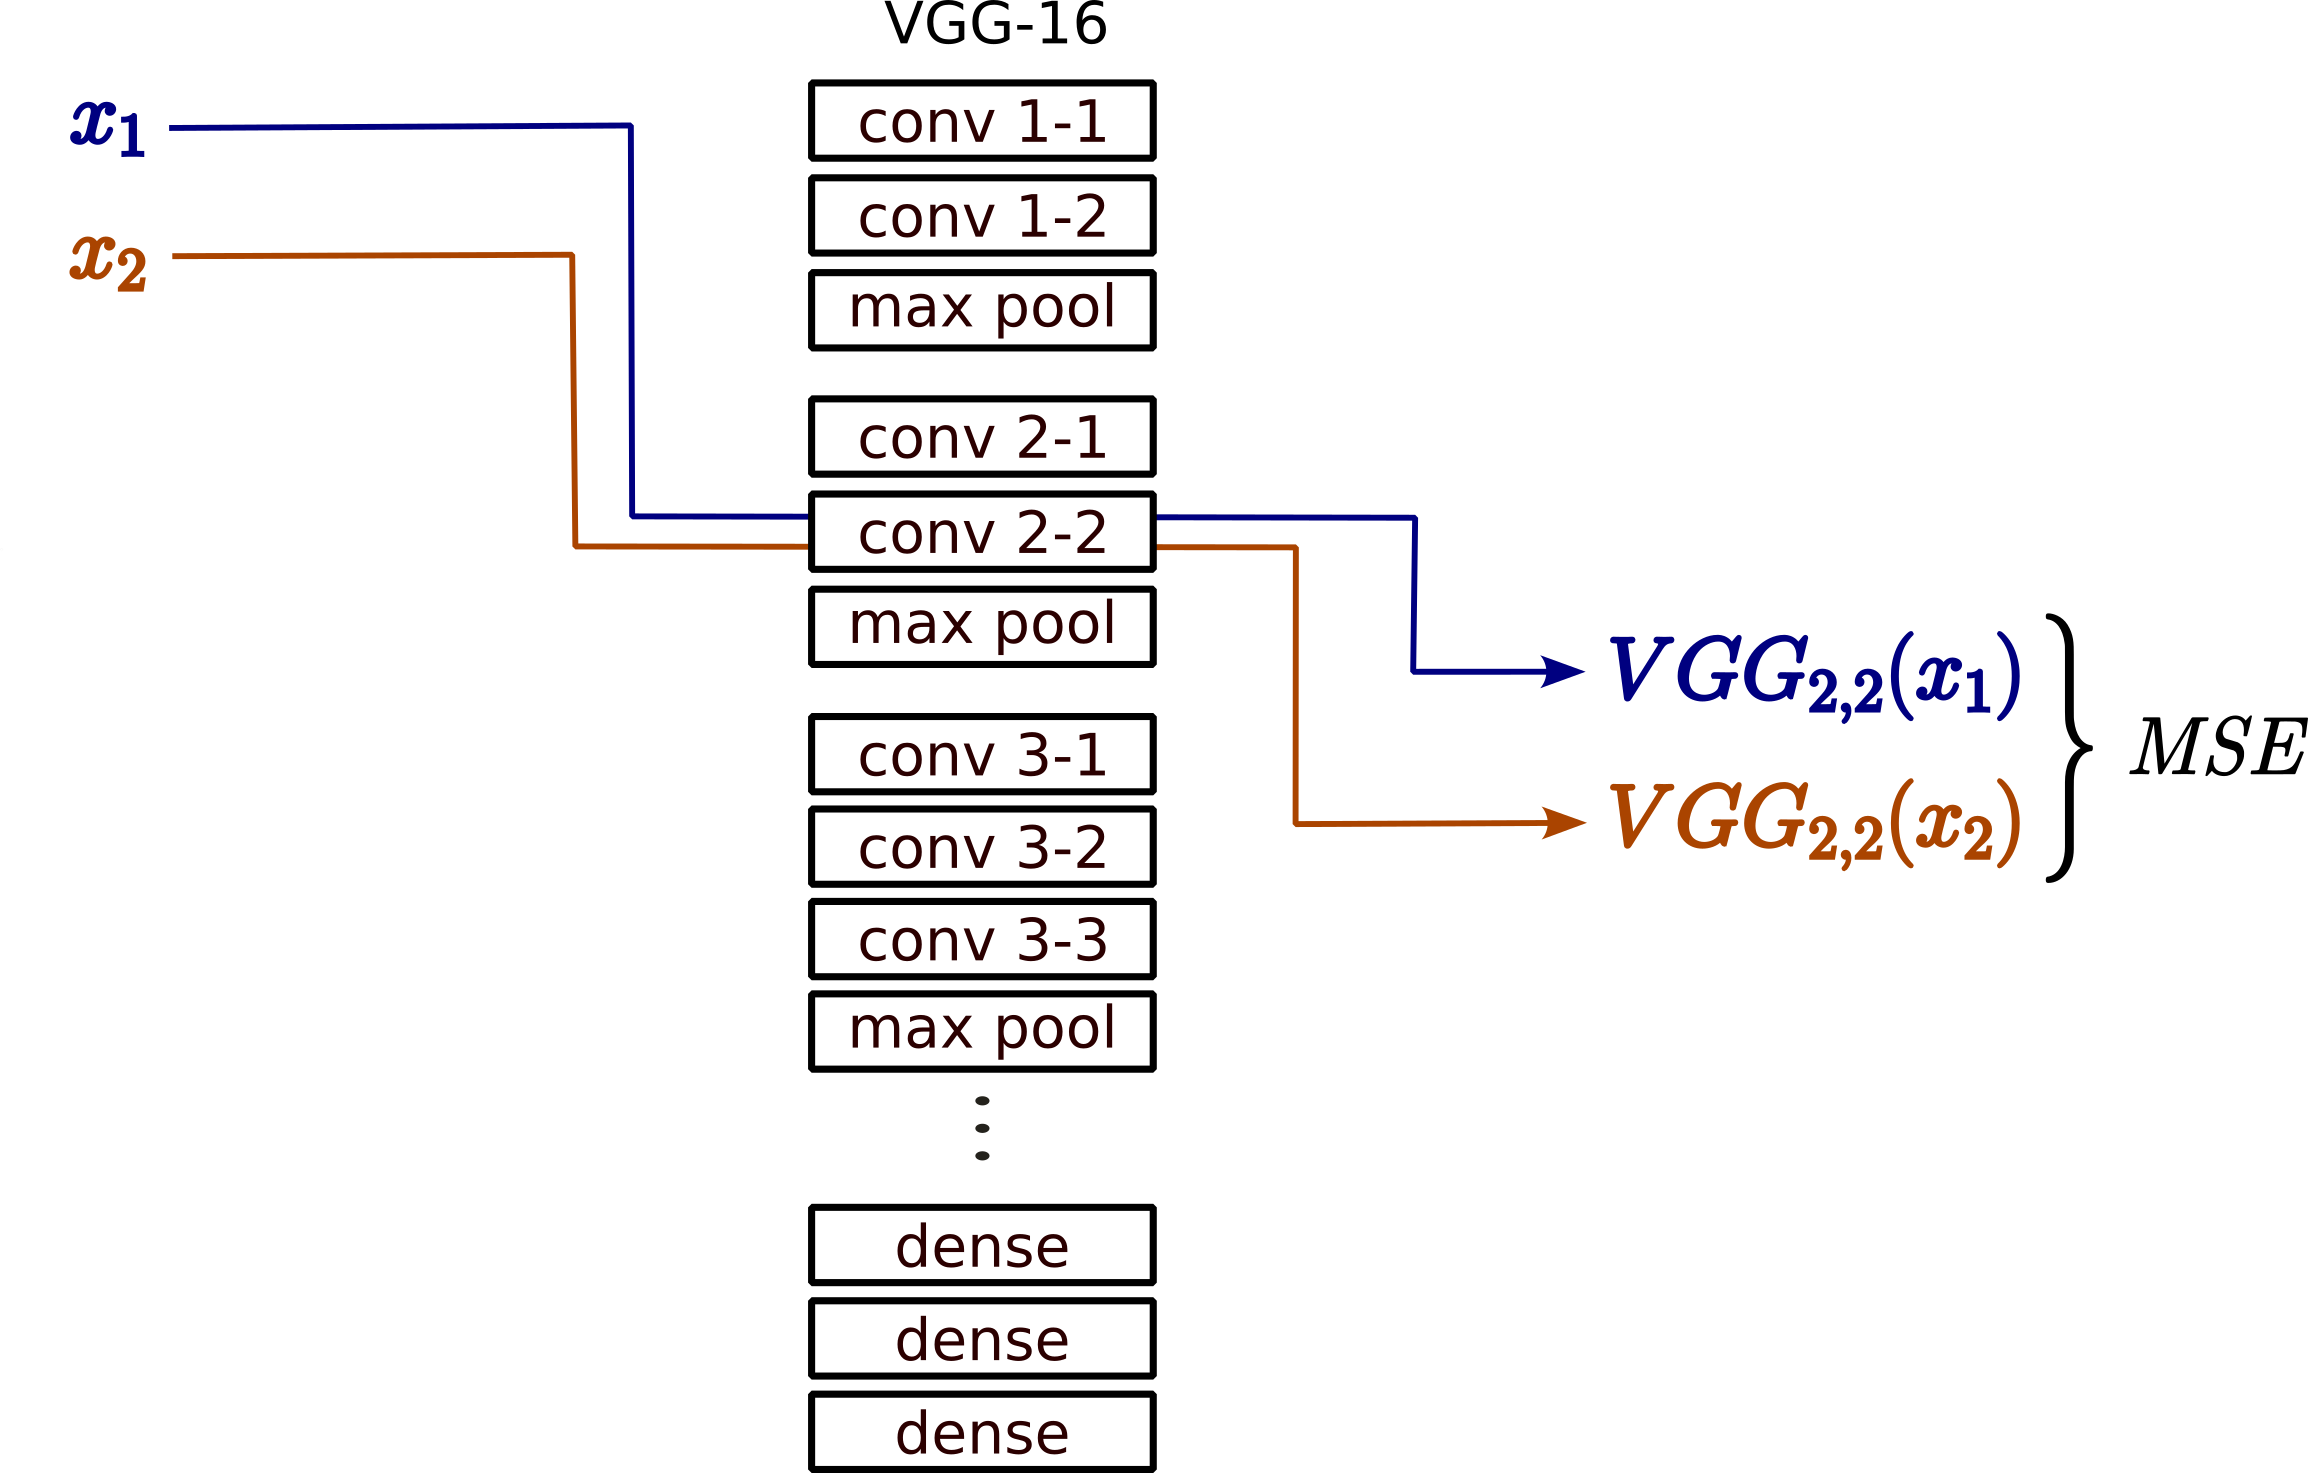
\includegraphics[width=0.75\textwidth]{vgg_qual.png}
  \end{figure}


\end{frame}


%%%%%%%%%%%%%%%%%%%%%%%%%%%%%%%%%%%%%%%%%%%%%%%%%%
\section{Perceptual quality: no reference image quality assessment}

%%%%%%%%%%%%%%%%%%%%%%%%%%%%%%%%%%%%
\begin{frame}{Classical methods}

  \begin{itemize}[<+->]
  \item Many methods: CBIQ, LBIQ, BLIINDS-II, DIVINE, BRISQUE, TMIO, NIQE~\cite{mittal_making_2013}
  \item Generally based on natural image statistics
  \end{itemize}


\end{frame}

%%%%%%%%%%%%%%%%%%%%%%%%%%%%%%%%%%%%
\begin{frame}{Inception score~\cite{salimans_improved_2016}}

\begin{figure}[ht]
  \centering
  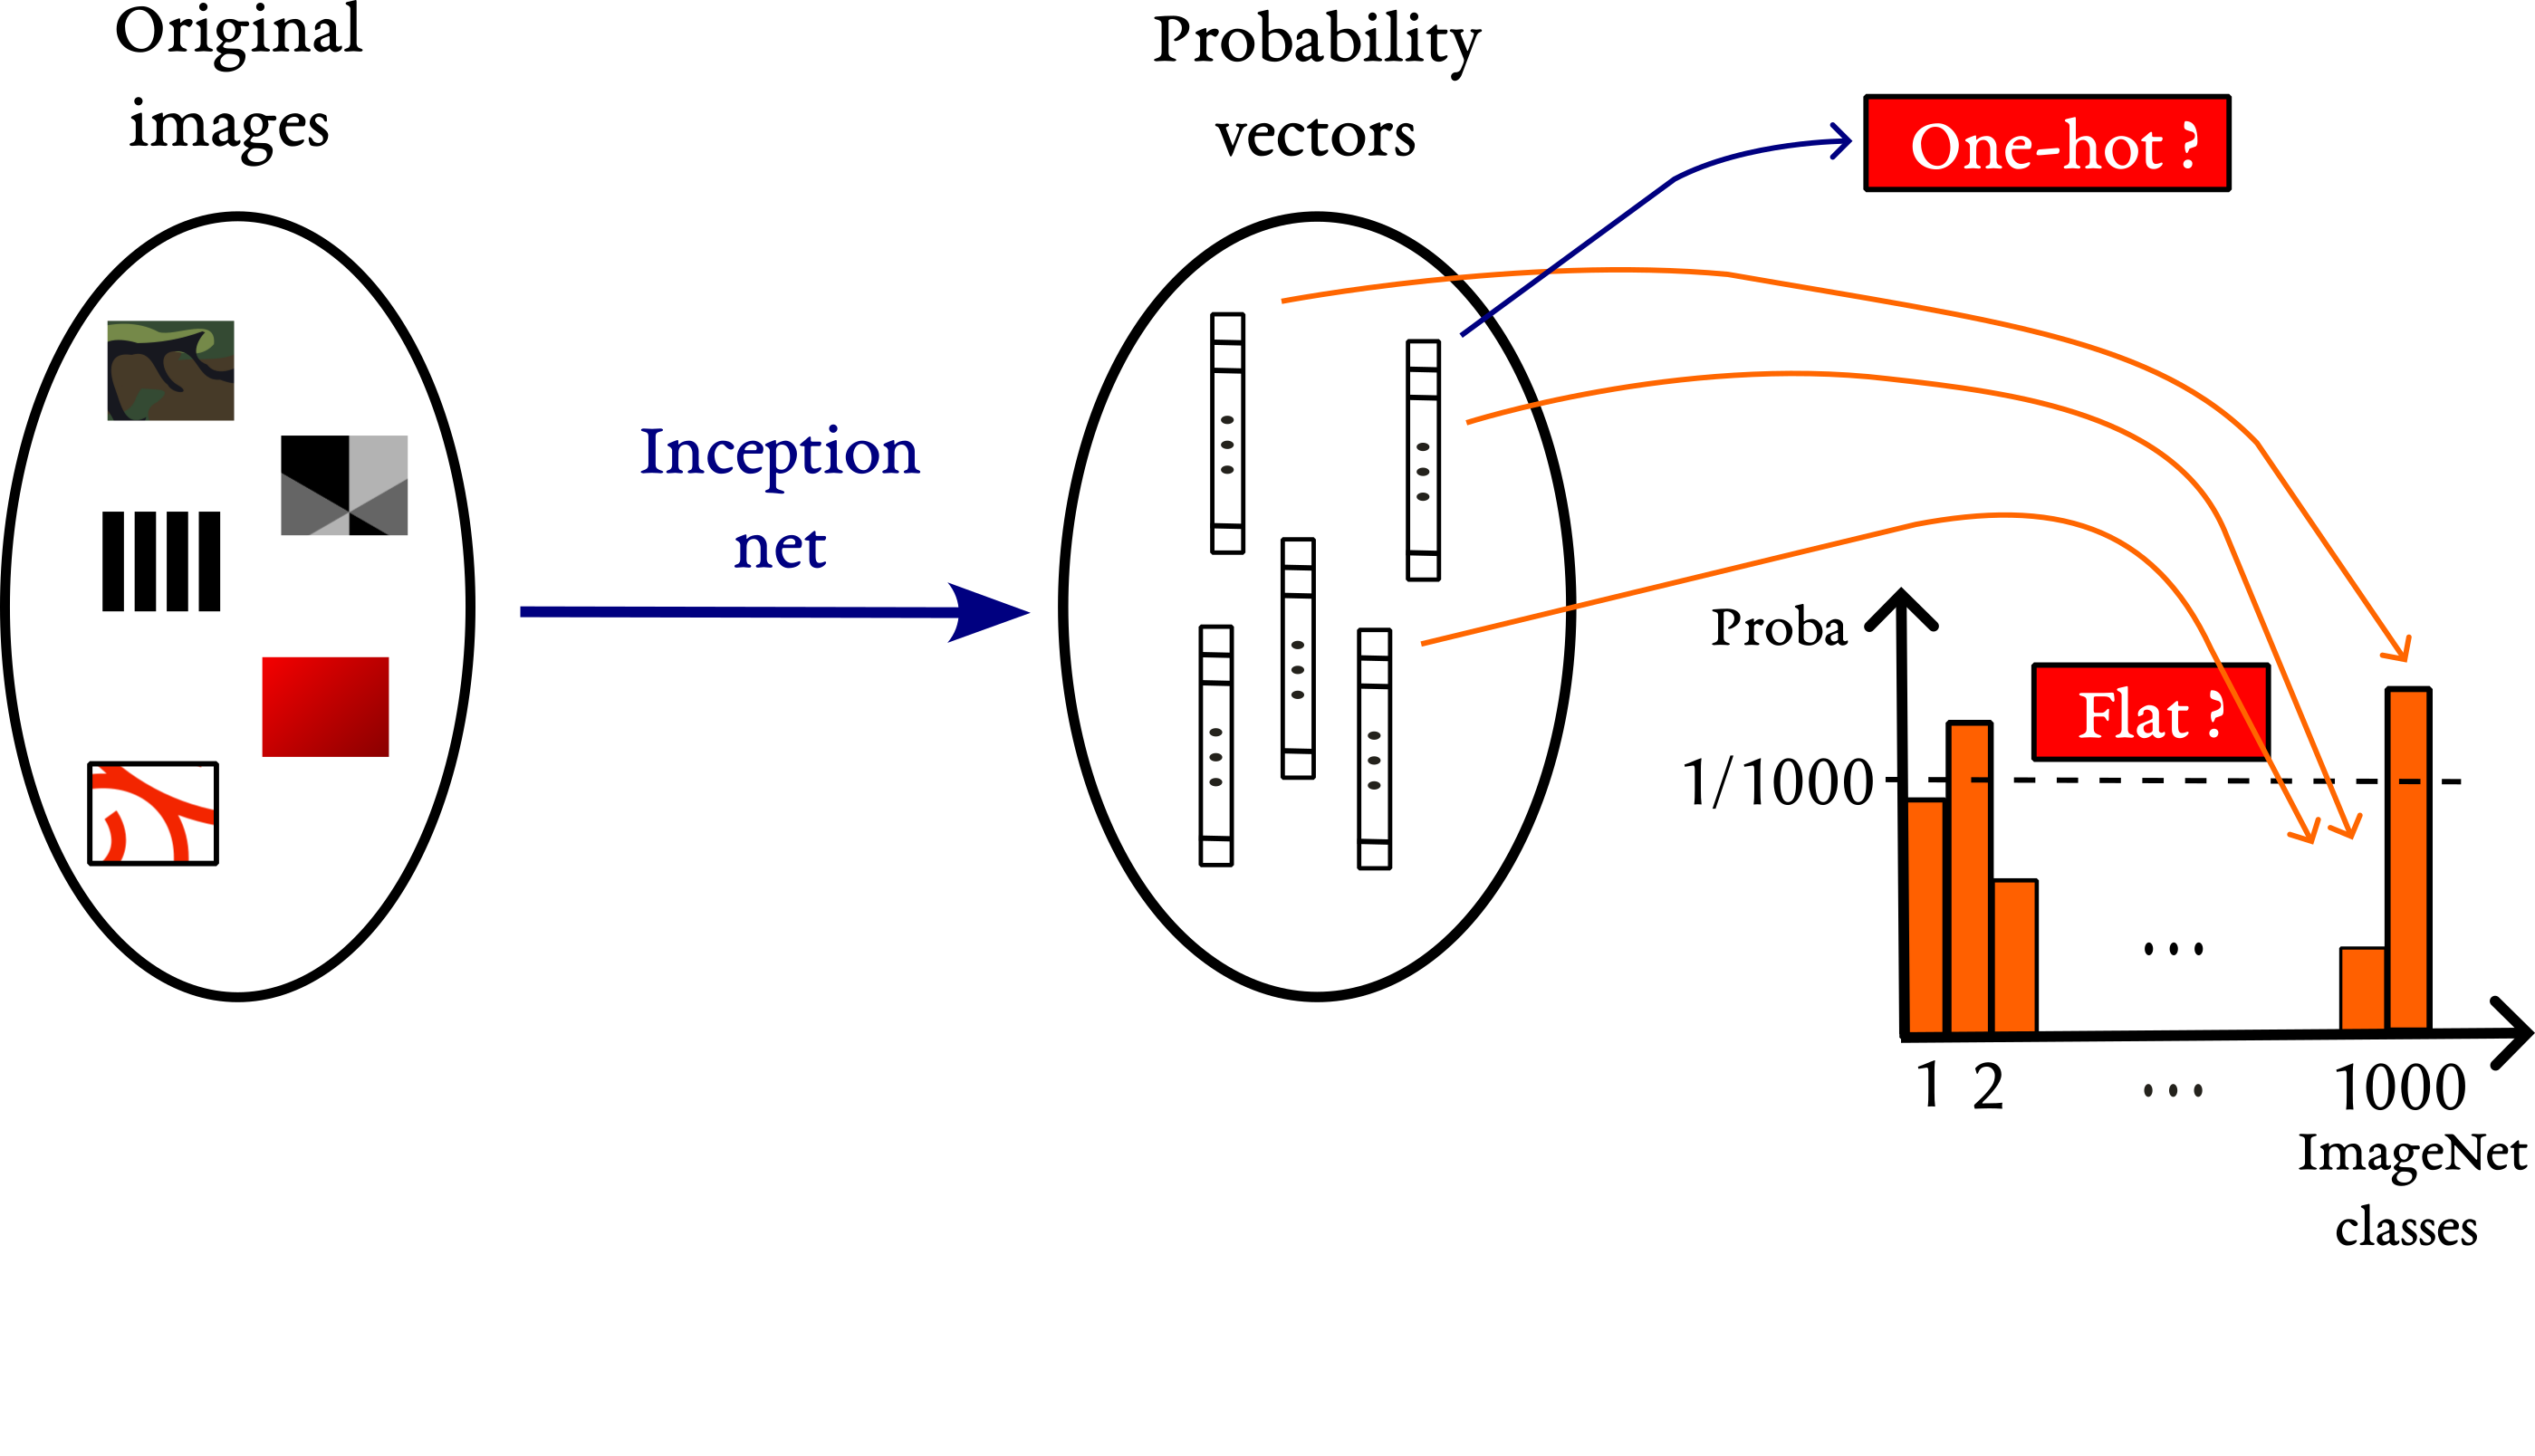
\includegraphics[width=0.8\textwidth]{inception_score}
\end{figure}


\end{frame}



%%%%%%%%%%%%%%%%%%%%%%%%%%%%%%%%%%%%
\begin{frame}{Fréchet inception distance~\cite{heusel_gans_2017}}

\end{frame}


%%%%%%%%%%%%%%%%%%%%%%%%%%%%%%%%%%%%%%%%%%%%%%%%%%
\section{Perception-distortion tradeoff}


%%%%%%%%%%%%%%%%%%%%%%%%%%%%%%%%%%%%
\begin{frame}{Observation~\cite{blau_perception-distortion_2018}}

  \begin{figure}[ht]
    \centering
    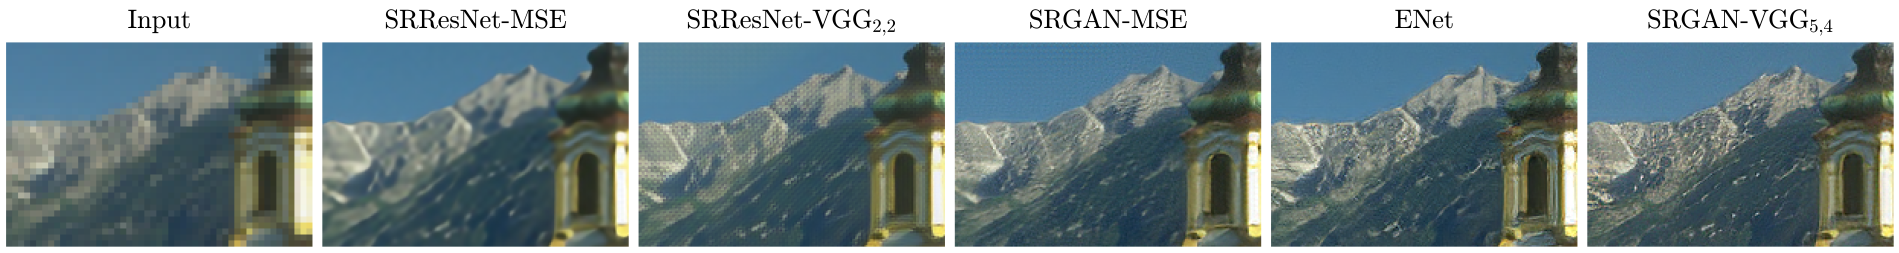
\includegraphics[width=\textwidth]{perception_distortion_tradeoff_illustration}
  \end{figure}

\end{frame}


%%%%%%%%%%%%%%%%%%%%%%%%%%%%%%%%%%%%
\begin{frame}{Perception-distortion tradeoff~\cite{blau_perception-distortion_2018}}

\begin{figure}[ht]
  \centering
  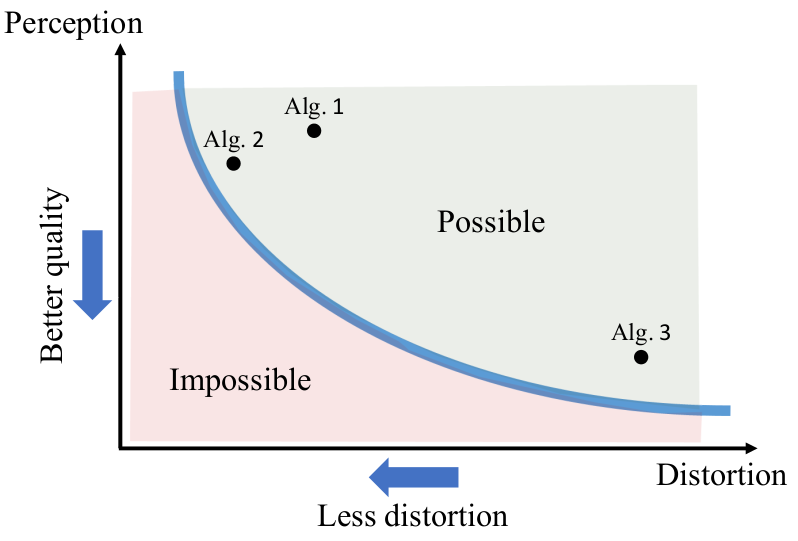
\includegraphics[width=0.8\textwidth]{impossible}
\end{figure}


\end{frame}

%%%%%%%%%%%%%%%%%%%%%%%%%%%%%%%%%%%%
\begin{frame}{Definitions}

\begin{itemize}[<+->]
\item $\Delta$ : distortion measure.
\item $d$ : divergence between distributions.
\end{itemize}

\pause

\begin{block}{Distortion, perception}
\begin{itemize}[<+->]
\item Distortion between $X$ and $\hat{X}$: $E[\Delta(X, \hat{X})]$
  \item Perception : $d(p_X, p_{\hat{X}})$
\end{itemize}

\end{block}



\end{frame}


%%%%%%%%%%%%%%%%%%%%%%%%%%%%%%%%%%%%
\begin{frame}{Theorem}

\begin{block}{Perception-distortion function}

  $$
  P(D) = min_{p_{\hat{X} | Y}} d(p_X, p_{\hat{X}})~~~ s.t.~~~ E(\Delta[X, \hat{X}]) \leq D
  $$

\end{block}

\pause

\begin{figure}[ht]
  \centering
  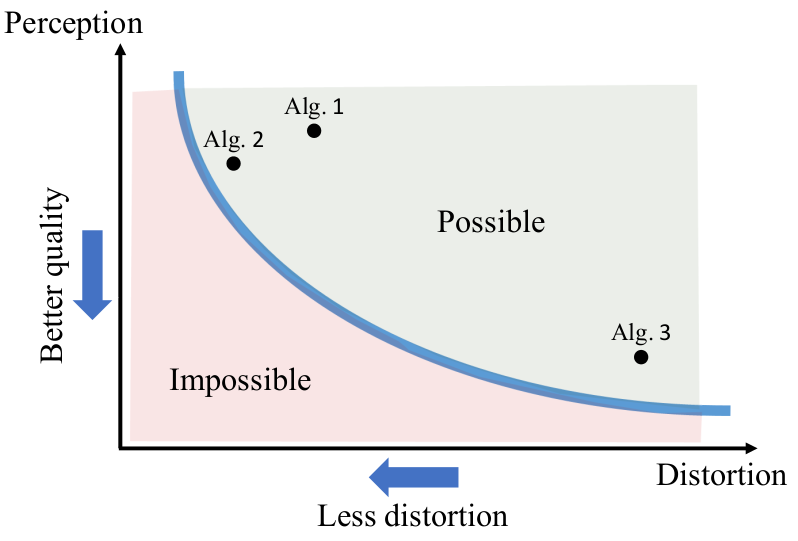
\includegraphics[width=0.4\textwidth]{impossible}
\end{figure}

\pause

\begin{block}{Theorem}
  If the divergence $d$ is convex in its second argument (which is the case for most common divergences) then $P(D)$ is monotonically non-increasing and convex.
\end{block}


\end{frame}



%%%%%%%%%%%%%%%%%%%%%%%%%%%%%%%%%%%%
\begin{frame}{Experiments}

\begin{figure}[ht]
  \centering
  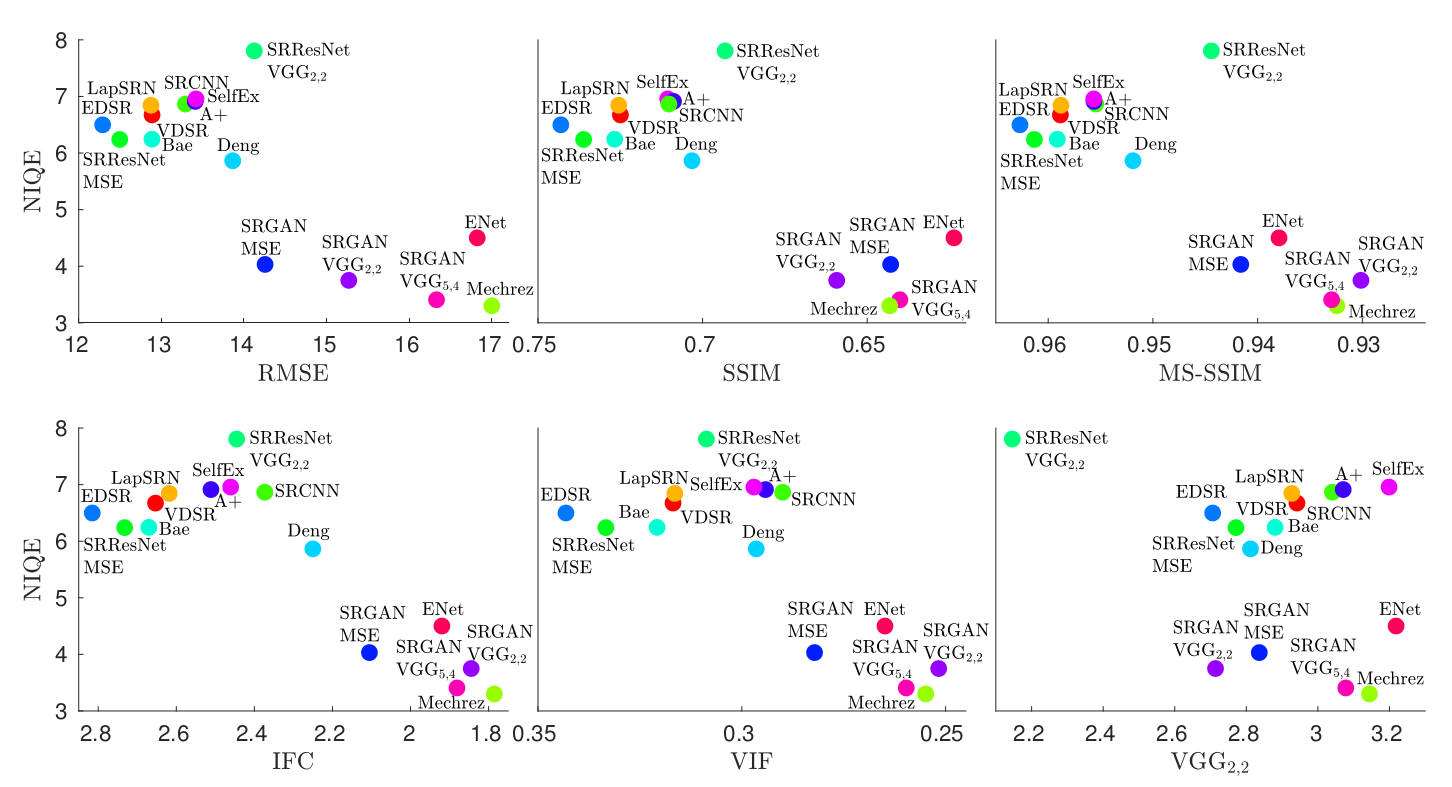
\includegraphics[width=\textwidth]{niqe}
\end{figure}


\end{frame}


%%%%%%%%%%%%%%%%%%%%%%%%%%%%%%%%%%%%%%%%%%%%%%%%%%
\section{Conclusion}

%%%%%%%%%%%%%%%%%%%%%%%%%%%%%%%%%%%%
\begin{frame}{Conclusion}

  \begin{itemize}[<+->]
  \item The tradeoff depends on the application
  \item In practice: choose an acceptable distortion, and try to optimize perceptual quality
\end{itemize}


\end{frame}



%%%%%%%%%%%%%%%%%%%%%%%%%%%%%%%%%%%%%%%%%%%%%%%%%%

%%%%%%%%%%%%%%%%%%%%%%%%%%%%%%%%%%%%%%%%%%%%%%%%%%
\section*{References}

%%%%%%%%%%%%%%%%%%%%%%%%%%%%%%%%%%%%%%%%%%%%%%%%%%

\frame[allowframebreaks]{

  \scriptsize

  \frametitle{References}

  %\bibliographystyle{amsalpha}
  %\bibliographystyle{apalike}

  \bibliography{../../edf.bib}

  \normalsize

}

\end{document}
